\documentclass[10pt,a4paper]{article}

\usepackage[utf8]{inputenc}
\usepackage[T1]{fontenc}
\usepackage[top=1.8cm,bottom=1.8cm,left=2.0cm,right=2.0cm]{geometry}
\usepackage{amsmath,amssymb}
\usepackage{graphicx}
\usepackage{booktabs}
\usepackage{microtype}
\usepackage{titlesec}
\usepackage{caption}
\usepackage[colorlinks=true,linkcolor=blue,citecolor=blue,urlcolor=blue]{hyperref}

% Crisp, compact headings for 1-page layout
\titlespacing\section{0pt}{4pt plus 1pt minus 1pt}{2pt plus 1pt minus 1pt}
\titleformat{\section}{\bfseries\normalsize}{\thesection.}{0.5em}{}

\title{\vspace{-0.8cm}\textbf{\large ATLAS: An Autonomous Neural AMR Solver for Stiff Multiscale Multiphysics in CAE Simulation Pipelines}\vspace{-0.3cm}}

\author{
    \textbf{Kartikeya Gangwar} \\
    \small Department of Mathematics, University of Delhi, Delhi 110007, India \\
    \small Email: \href{mailto:kartikeyagangwar@proton.me}{\texttt{kartikeyagangwar@proton.me}}
}
\date{\vspace{-0.7cm}}

\begin{document}

\maketitle
\thispagestyle{empty}

\noindent\textbf{Abstract.} Physics-Informed Neural Networks (PINNs) hold strong promise as surrogate solvers in Computer-Aided Engineering (CAE). However, their industrial deployment is hindered by optimization failure in stiff, multi-scale, and convection-dominated regimes. We introduce \textbf{ATLAS} (Adaptive Tiling of Localized Anisotropic Subspaces), an autonomous neural Adaptive Mesh Refinement (AMR) framework. ATLAS detects localized gradient conflict online via batched reverse-mode autodiff (\texttt{torch.func.vmap}) at line-rate, dynamically cleaves localized anisotropic subdomains governed by bandwidth $\boldsymbol{\Sigma}$, and blends solutions seamlessly under a $C^\infty$ Partition of Unity (PoU) without interface continuity loss penalties. Evaluated on canonical CAE benchmarks, ATLAS reduces test errors by up to $418.5\times$ over monolithic PINNs and resolves recirculating vortices with an order-of-magnitude lower error.

\section{Industrial Motivation \& Parameter Entanglement Barrier}
Modern CAE workflows (e.g., Ansys, Siemens Simcenter, OpenFOAM) rely on Adaptive Mesh Refinement to concentrate degrees of freedom around steep gradients, boundary layers, and shocks without manual re-meshing. In contrast, standard PINNs map the entire domain through a monolithic parameter vector $\Theta \in \mathbb{R}^P$. When the domain contains disparate physical regimes (e.g., localized shear vs.\ quiescent flow), collocation points backpropagate opposing gradients ($\langle \mathbf{g}_1, \mathbf{g}_2 \rangle < 0$), causing destructive gradient interference, artificial numerical dissipation, and boundary divergence. Multi-objective projection schemes (PCGrad, CAGrad) share the same weights and suppress essential constraints, while Cartesian domain decomposition methods (XPINN, FBPINN) suffer from exponential grid explosion $\mathcal{O}(K_0^d)$ or fragile interface penalties.

\section{The ATLAS Methodological Framework}
ATLAS resolves parameter entanglement through three core innovations:
\begin{enumerate}\setlength{\itemsep}{0pt}\setlength{\parskip}{0pt}
    \item \textbf{Vectorized Online Conflict Profiling (\texttt{torch.func.vmap}):} Per-sample gradients and their Gram matrix $\mathbf{K}_k = \mathbf{G}_k \mathbf{G}_k^T$ are evaluated across collocation batches in $12\text{--}18$\,ms on GPU ($47\times\text{--}83\times$ faster than serial loops). Subspaces exceeding conflict thresholds ($\overline{\mathcal{C}}_k < 0.10$ or $\hat{\rho}_k > 0.20$) automatically spawn child centroids at coordinates of peak PDE residual.
    \item \textbf{Dimension-Normalized Anisotropic Partition of Unity:} Subspaces are synthesized via $\hat{u}(\mathbf{x}) = \sum_{k=1}^N \psi_k(\mathbf{x})\Phi_k(\tilde{\mathbf{x}}_k; \Theta_k)$, with normalized Gaussian gates $\psi_k(\mathbf{x}) = w_k(\mathbf{x})/\sum_j w_j(\mathbf{x})$ and coordinate bandwidths $\sigma_i = \gamma \Delta x_i$ ($\gamma \in [0.20, 0.30]$). Disjoint parameter blocks $\Theta_k$ eliminate inter-subspace gradient clashing, while $C^\infty$ blending removes all interface loss penalties.
    \item \textbf{Two-Stage Discover-and-Deploy Protocol:} A lightweight Stage~1 probe ($32 \times 2$ MLP, $\sim 1.1\text{K}$ parameters/subspace) discovers the parsimonious count $N^*$ and centroid coordinates. Stage~2 then trains a clean production model polished by joint second-order Quasi-Newton (Combined Global L-BFGS).
\end{enumerate}

\section{Empirical Validation on Key CAE Benchmarks}
\begin{minipage}{0.48\textwidth}
\centering
\captionof{table}{\textbf{Quantitative Benchmark Test Loss.} Evaluated on $10{,}000$ held-out test points.}
\label{tab:cae_results}
\scriptsize
\begin{tabular}{lcccc}
\toprule
\textbf{Benchmark Problem} & \textbf{Standard PINN} & \textbf{PCGrad} & \textbf{ATLAS (Ours)} & \textbf{Gain} \\
\midrule
1D Burgers Shock ($\nu=0.01/\pi$) & $3.12 \times 10^{-1}$ & $6.12 \times 10^{0}$ & $\mathbf{4.82 \times 10^{-2}}$ & $\mathbf{6.5\times}$ \\
2D Convection ($\mathrm{Pe}=10^3$) & $1.64 \times 10^{0}$ & $4.58 \times 10^{0}$ & $\mathbf{1.68 \times 10^{-2}}$ & $\mathbf{97.9\times}$ \\
2D Helmholtz Wave ($k=4\pi$) & $8.61 \times 10^{2}$ & $3.15 \times 10^{3}$ & $\mathbf{2.06 \times 10^{0}}$ & $\mathbf{418.5\times}$ \\
2D Cavity Flow ($\mathrm{Re}=100$) & $2.91 \times 10^{-1}$ & $3.08 \times 10^{-1}$ & $\mathbf{1.19 \times 10^{-1}}$ & $\mathbf{2.4\times}$ \\
\bottomrule
\end{tabular}
\end{minipage}
\hfill
\begin{minipage}{0.49\textwidth}
\centering
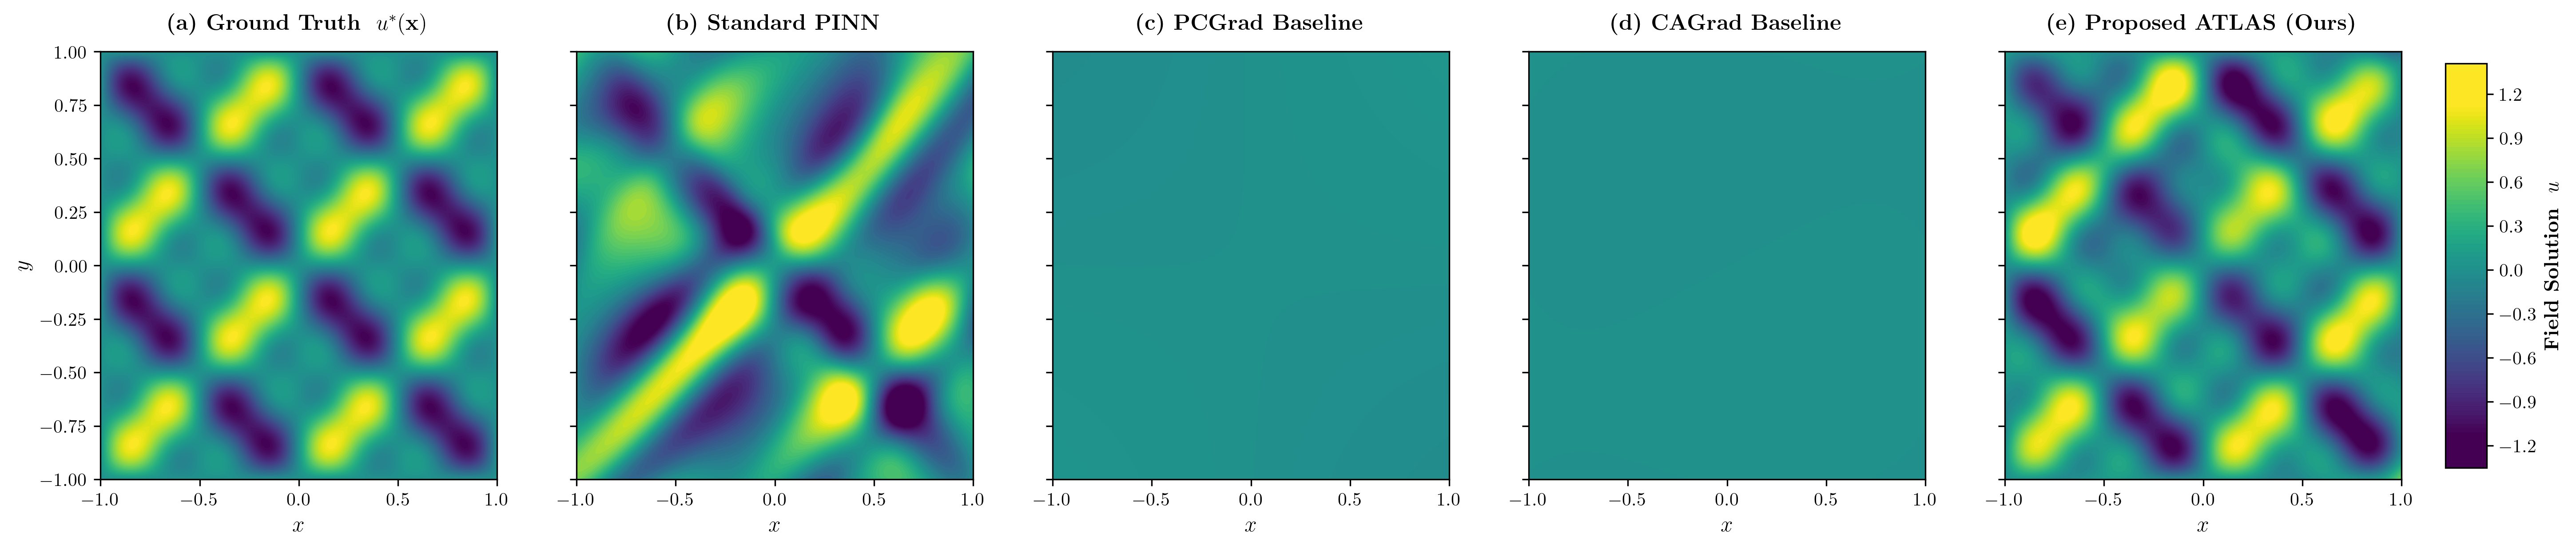
\includegraphics[width=\textwidth]{helmholtz2d_solutions.png}
\captionof{figure}{\textbf{2D Helmholtz ($k=4\pi$).} ATLAS isolates 16 extrema into 21 subspaces, achieving $418.5\times$ error reduction.}
\label{fig:helmholtz_short}
\end{minipage}

\vspace{0.2cm}
\noindent\textbf{Key Findings:} In high-frequency Helmholtz scattering ($k=4\pi$), monolithic PINNs trap in spectral bias while ATLAS isolates wave lobes ($418.5\times$ error reduction). In 2D Cavity Navier-Stokes ($\mathrm{Re}=100$), ATLAS concentrates 23 subspaces near the moving lid and corner recirculation zones, reducing streamfunction relative $L^2$ error by $9.5\times$ ($7.17\%$ vs.\ $68.0\%$).

\section{CAE Industry Readiness \& Open-Source Availability}
ATLAS is implemented in pure PyTorch with zero external dependencies and supports multi-GPU parallelization. Complete code, checkpoints, and automated benchmark runners are available at: \url{https://github.com/KartikeyaGangwar/atlas-neural-amr}.

\vspace{0.1cm}
{\scriptsize
\noindent\textbf{References:} 
[1] Raissi et al., \textit{J. Comput. Phys.}, 378:686--707, 2019. 
[2] Krishnapriyan et al., \textit{NeurIPS}, 34:26548--26560, 2021. 
[3] Gangwar, \textit{Zenodo}, DOI: 10.5281/zenodo.22132799, 2026.
}

\end{document}
